\documentclass{article}
\usepackage[polish]{babel}
\usepackage[T1]{fontenc}
\usepackage{lmodern}
\usepackage[utf8]{inputenc}
\usepackage{graphicx}
\usepackage{bookmark}
\usepackage{float}
\usepackage{hyperref}
\usepackage[bottom=1.5cm, right=2.5cm, left=2.5cm, top=1.5cm]{geometry}
\graphicspath{{../pliki}}



\title{%
  Cyberbezpieczeństwo - laboratoria 12 \\
  \large Wykorzystanie podatności - eskalacja uprawnień}
\author{Patryk Łuszczek 272707}
\date{\today}
\begin{document}
\maketitle
\newpage
\section*{Adresy maszyn wirtualnych}
\begin{itemize}
    \item Kali Linux - 10.0.4.4
    \item Metasplotable - 10.0.4.7
\end{itemize}
\section*{Co to jest reverse shell?}
Reverse shell to technika pozwalająca na wykonanie m.in. zdalnego ataku. Polega na ustanowieniu połączenia z maszyną ofiary
"od środka", przy czym maszyna atakującego pełni role serwera, do którego będzie podłączone urządzenie ofiary. Dzięki tej zależności, jest możliwe ominięcie wielu zabezpieczeń sieciowych, takich jak zapory sieciowe, które blokują połączenia przychodzące
ale zezwalają na ruch wychodzący. Pozwala to na pobranie szkolidiwego oprogramowania na maszynę ofiary, szkodliwego kodu oraz jego uruchomienie.
\section*{Dlaczego ważne jest nadanie odpowiednich uprawnień kontom użytkowników, w
  szczególności kontom używanym domyślnie przez usługi działające w systemach}

Dzięki ustawieniu ograniczonych uprawnień kontom użytkowników mają oni dostęp wyłącznie do zasobów niezbędnych do wykonywania swoich zadań.
Atak na takie konto jest mniej szkodliwy, ponieważ w przypadku jego przejęcia intruz uzyskuje dostęp jedynie do ograniczonych zasobów. Należy również zwrócić uwagę na konta używane przez różnego rodzaju usługi działające w systemie,
ponieważ jeśli posiada ona luki w zabezpieczeniach mogą stać się bardzo atrakcyjnym celem ataków.

\section*{Skanowanie nmap}
\begin{figure}[H]
    \centering
    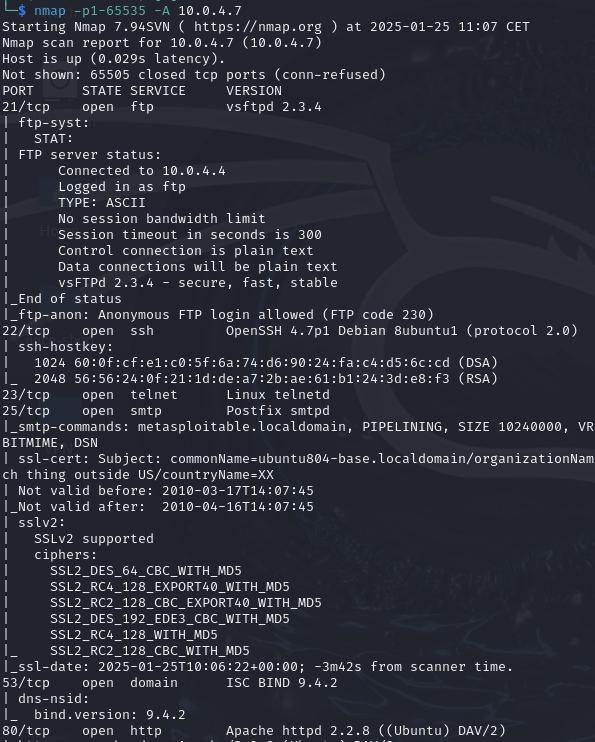
\includegraphics[width=0.8\textwidth]{skanowanie_tcp.png}
    \caption{Wynik skanowania nmap}
\end{figure}
Jak można zauważyć na Metasplotable jest uruchomione wiele serwisów. Interesującym nas serwisem jest serwer FTP działający na porcie 21 (TCP).
Serwerem FTP na mszynie jest vsFTPd w wersji 2.3.4. Ta wersja serwera jest podatna na atak pozwalający na zdalne wykonywanie kodu poprzez otworzenie portu 6200 za pomocą logowania netcat do portu z nsFTPd z użyciem nazwy użytkownika zawierającej znak \texttt{:)} (\href{https://nvd.nist.gov/vuln/detail/CVE-2011-2523}{CVE-2011-2523}).
Obecnie skanowanie nmap nie wykryło otwartego portu 6200.
\section*{Próba otworzenia portu 6200 i połączenia się z maszyną}
\begin{figure}[H]
    \centering
    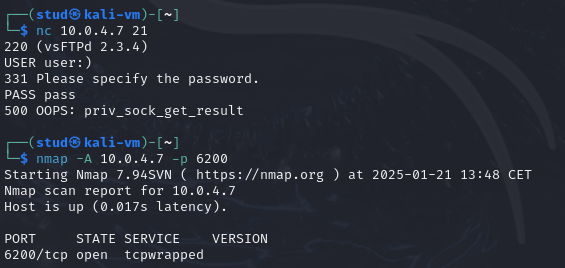
\includegraphics[width=0.8\textwidth]{otwarcie_portow_6200.png}
    \caption{Otwarcie portu 6200}
\end{figure}
Jak można zauważyć logowanie przy użyciu nazwy użytkownika zawierającej znak \texttt{:)} i dowolnym hasłem pomyślnie otworzyło port 6200.
\begin{figure}[H]
    \centering
    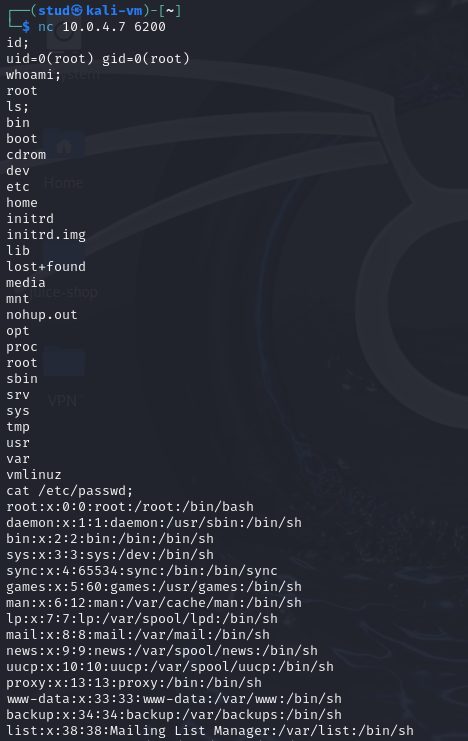
\includegraphics[width=0.8\textwidth]{nc_6200.png}
    \caption{Połączenie z portem 6200}
\end{figure}
Pomyślnie udało się połączyć z portem 6200. Uzyskano prawa roota, pozwola to na wgląd do plików takich jak np. hasła i użytkonicy.
\section*{Distccd}
Distccd to serwer kompilacji kodu C/C++/Obj-C równolegle na kilku maszynach pracyjących w sieci. Standardowo usługa uruchomiona jest na porcie 3632.
\begin{figure}[H]
    \centering
    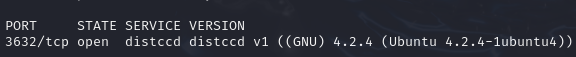
\includegraphics[width=0.8\textwidth]{distccd.png}
\end{figure}
Za pomocą środowiska metasploit odnaleziono exploit dla disccd o nazwie $\texttt{exploit/unix/misc/distcc\_exec}$
\begin{figure}[H]
    \centering
    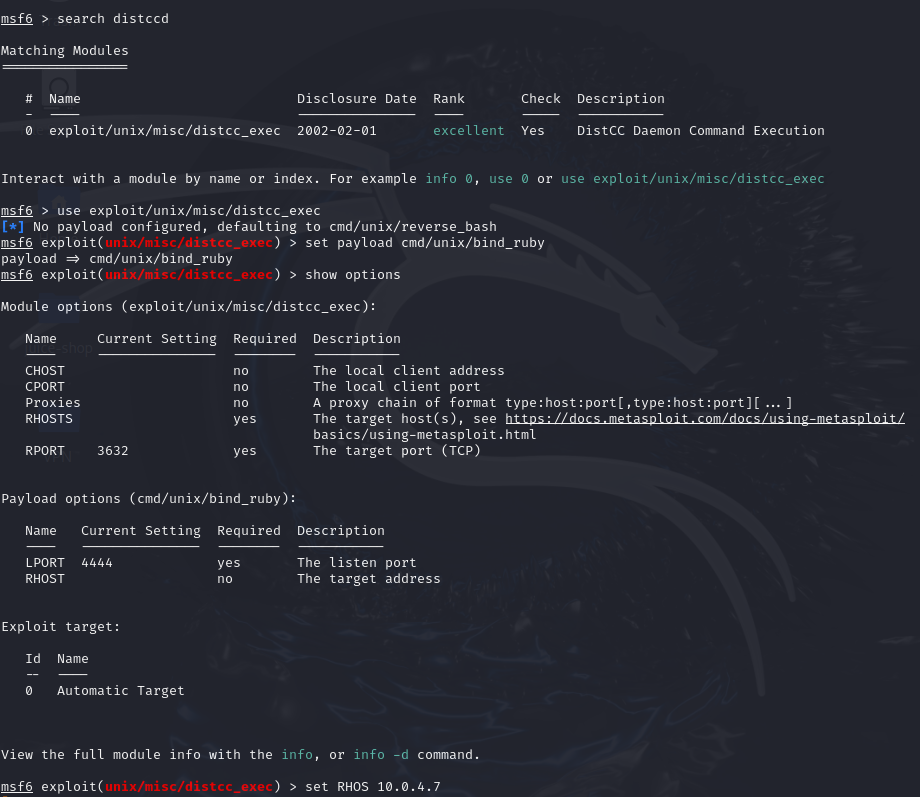
\includegraphics[width=0.8\textwidth]{explot.png}
\end{figure}
\begin{figure}[H]
    \centering
    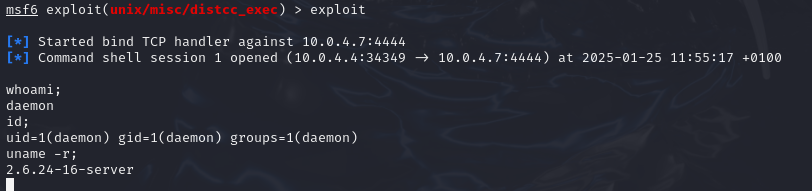
\includegraphics[width=0.8\textwidth]{explot_id_uname.png}
\end{figure}
Jak można zauważyć udało się uzyskać dostęp do maszyny, jednak bez praw roota.
Za pomocą luki CVE-2009-1185 można wykorzystać podatność udev w wersji przed 1.4.1 na uzyskanie praw roota.

W bazie exploit-db odnaleziono exploita wykorzystującego lukę \href{https://www.exploit-db.com/exploits/8572}{Linux Kernel 2.6 (Gentoo / Ubuntu 8.10/9.04) UDEV < 1.4.1 - Local Privilege Escalation} dzięki, której
będziemy mogli uzyskać uprawnienia roota.

Pobrany exploit został przeniesiony do folderu /var/www/html a następnie została włączona usługa apache2.service w celu udostępnienia exploitu na maszyne ofiary.
Za pomocą msfconsole pobrano plik z kodem, skompilowano do pliku wykonywalnego, stworzono skrypt, który po uruchomieniu exploita da nam uprawnienia roota na maszynie kali oraz włączono nasłuchiwanie na porcie 31337.
\begin{figure}
    \centering
    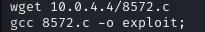
\includegraphics[width=0.5\textwidth]{wykonane_exploita.png}
    \caption{Przygotowanie exploitu}
\end{figure}

Ostatecznie uruchomienie exploita na maszynie ofiary zakończyło się sukcesem - uzyskano uprawnienia roota.

\begin{figure}[H]
    \centering
    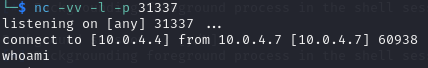
\includegraphics[width=0.5\textwidth]{udany_exploit.png}
    \caption{Uzyskanie uprawnień roota}
\end{figure}
\begin{figure}[H]
    \centering
    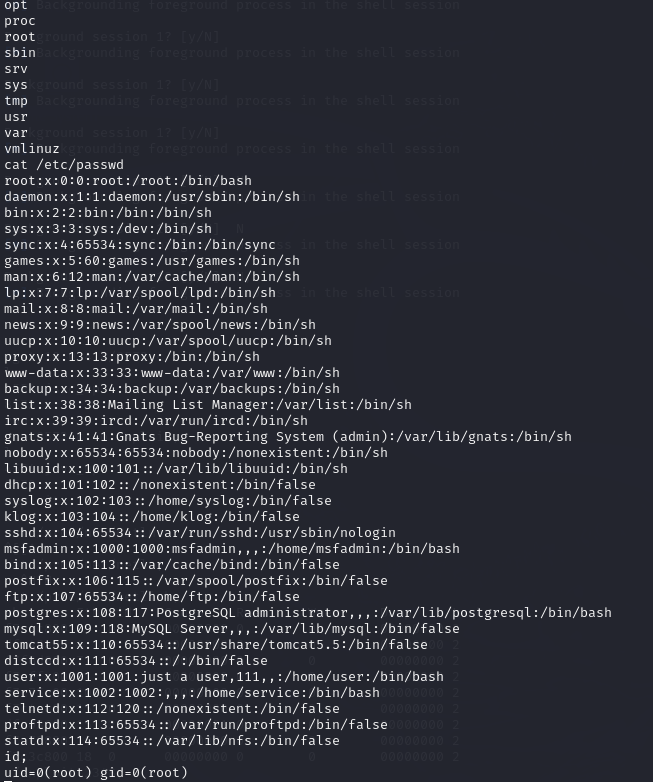
\includegraphics[width=0.5\textwidth]{root.png}
\end{figure}

\end{document}